\documentclass{article}
\usepackage{listings}
\usepackage{amsfonts}
\usepackage{latexsym}
\usepackage{fullpage}
\usepackage{graphicx}
\usepackage{paralist}
\usepackage{tikz-timing}

\lstdefinelanguage{VHDL}{
  morekeywords={
    library,use,all,ENTITY,IS,PORT,IN,OUT,end,architecture,of,
    begin,and, ARCHITECTURE, IF, THEN, SIGNAL,END, PROCESS
  },
  morecomment=[l]--
}

\usepackage{xcolor}
\colorlet{keyword}{blue!100!black!80}
\colorlet{comment}{green!90!black!90}
\lstdefinestyle{vhdl}{
  language     = VHDL,
  basicstyle   = \ttfamily\scriptsize,
  keywordstyle = \color{keyword}\bfseries\ttfamily,
  commentstyle = \color{comment}\ttfamily,	
  tabsize=1
}

\renewcommand{\lstlistingname}{Code}

% Default margins are too wide all the way around. I reset them here
\setlength{\topmargin}{-.5in}
\setlength{\textheight}{9in}
\setlength{\oddsidemargin}{.125in}
\setlength{\textwidth}{6.25in}


%\let\oldenumerate\enumerate
%\renewcommand{\enumerate}{
  %\oldenumerate
  %\setlength{\itemsep}{1pt}
  %\setlength{\parskip}{0pt}
  %\setlength{\parsep}{0pt}
%}


\begin{document}
\title{Organization of Digital Computer Lab \\ EECS112L/CSE 132L}
\author{\textbf{Assignment 1 }\\ \textbf{Working with CAD tools} \\ \\
prepared by: \\ Student name: \\Jack Melcher \\Student ID: \\67574625~\\ \\ 
EECS Department\\ Henry Samueli School of Engineering \\ University of California, Irvine \\ \\
{January, 6, 2016}} 


\date{}
\maketitle

\section{What I've learned}
	\subsection{QuestaSim}
		\begin{itemize}
			\item Questasim can only be used on zuma or crystalcove Unix servers
			\item How to setup a project that uses Questasim
			\item Install Questasim for my use on the server for the project
			\item Compile the VHDL(.vhd)  design files and the System Verilog(.sv) testbench files
			\item Optimize the VHDL design
			\item Simulate the design
			\item View the waveform
		\end{itemize}
	\subsection{Cadence}
		\begin{itemize}
			\item Cadence can only be used on malibu or vivian Unix servers
			\item Enable Cadence for use on my account
			\item How to setup a project that uses Cadence
			\item Compile the VHDL(.vhd)  design files and the System Verilog(.sv) testbench files
			\item Elaborate the VHDL design
			\item Simulate the design
			\item View the waveform
		\end{itemize}
		
\section{MentorGraphics QuestaSim toolset}
 
	\subsection{Simulation waveform}
	
	\bfseries{Simulation Waveform is as follows:} \\
	
	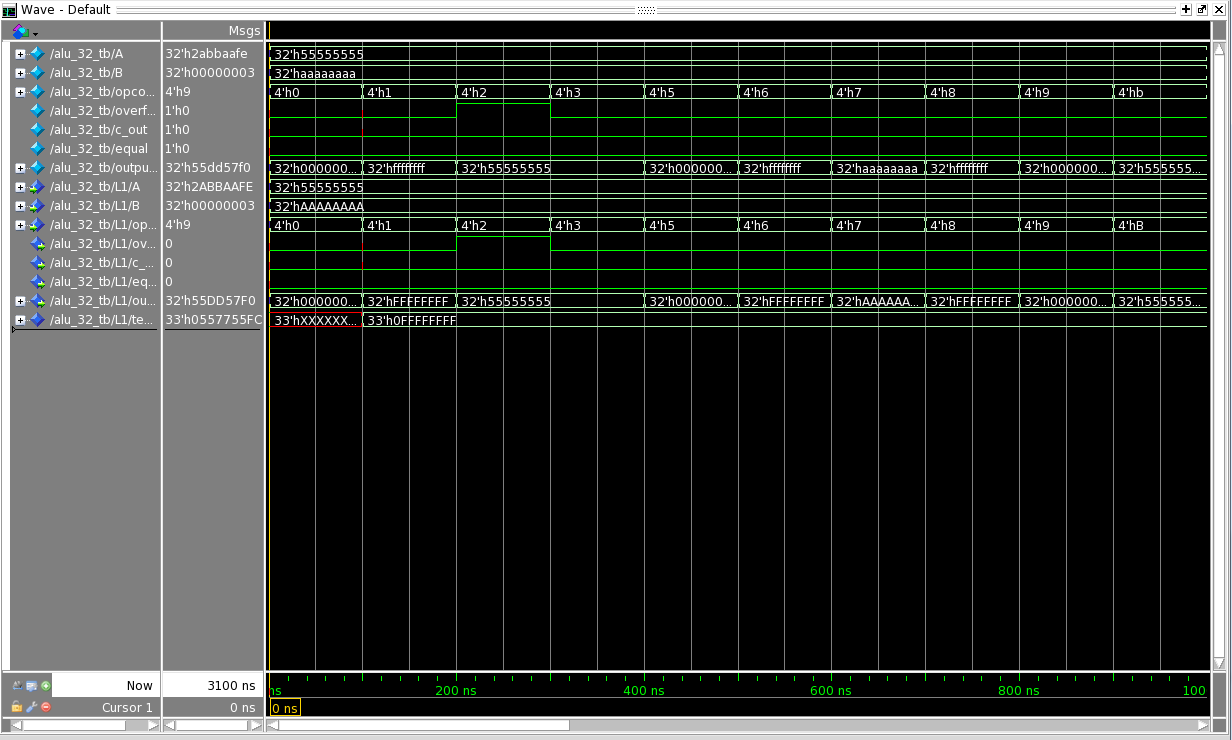
\includegraphics[width=0.8\columnwidth]{waveform_questasim.png}

\section{Cadence Incisive toolset}

	\subsection{Simulation waveform}

	\bfseries{Simulation Waveform is as follows:} \\

	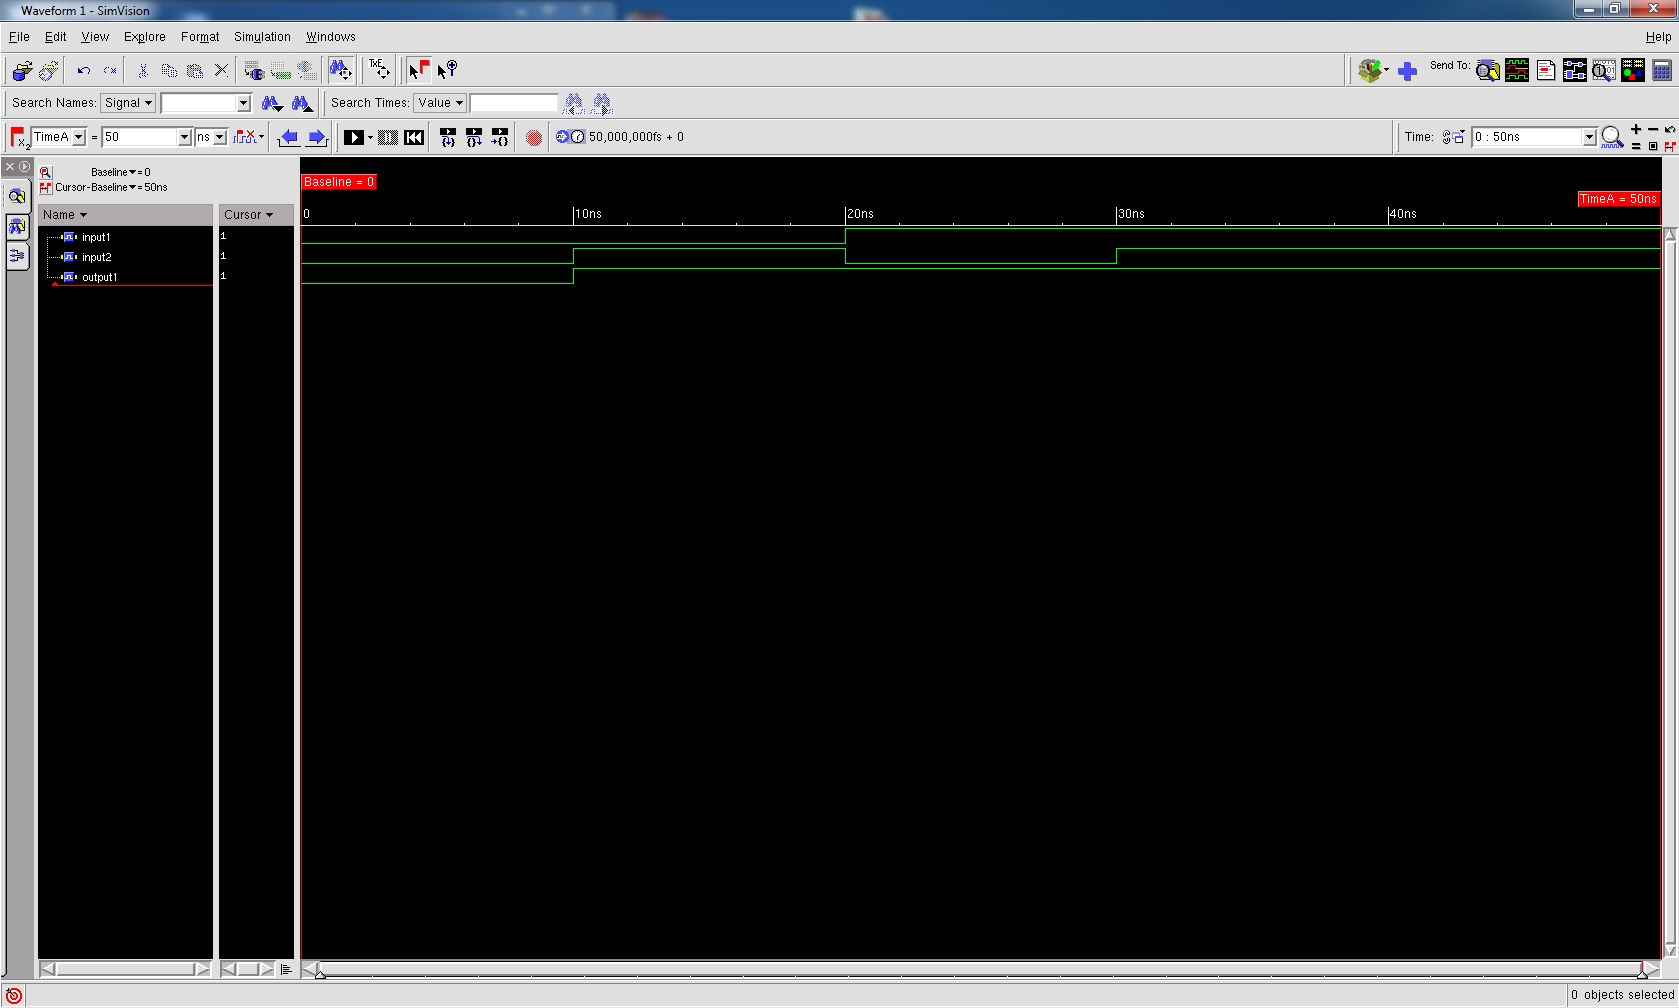
\includegraphics[width=0.8\textwidth]{waveform_cadence.png}

\section{Conclusion}

	I would prefer to use MentorGraphics QuestaSim toolset for the 112L course and because I found the compiling and optimization of the code to be easier and the display of the waveform more intuitive.


\end{document}
